\chapter{Présentation du stage}

\section{Le sujet}
\label{le-sujet}
Le titre du sujet du stage était initialement \enquote{\textit{Developer C++/Qt.
work on a challenging and immersive 360 video software}}.\\
Bien que très général, le domaine de l'entreprise se trouvait être très intéressant
et durant l'entretien qui s'est déroulé à la mi-mai, quelques sujets ont été
développés~: M. Burtey a proposé de travailler sur le Player d'une part,
à la suite d'Alexis Pontin et pour terminer son travail, et d'une autre part de
travailler au développement du nouveau produit VideoStitch Live, renommé par la
suite en Vahana VR, qui allait débuter dans quelques semaines.\\
M. Burtey n'était pas encore certain du lancement du développement de Vahana VR, 
et envisageait également à la conception du \textit{stitch} stéréoscopique 3D\footnote{Qui
consiste, brièvemenent, en la conception de deux équirectangulaires pour la même
scène filmée~: un pour chaque oeil en exploitant l'effet de la parallaxe, recréant 
un effet de relief\cite{videostitch-stereo}
\cite{image-stereoscopique}}, il me proposa également de travailler au développement
de la prise en charge de la 360 stéréo dans Videostitch Studio. Le sujet final serait
décidé la première semaine du stage.\\
\newline
Le stage fut finalement précédé par un contrat à temps partiel de 7 semaines, les missions retenues
se sont alors simplement étendues du début du CDD à la fin du stage, c'est-à-dire 
7 mois.\\
Le sujet réel a donc été arrêté à deux missions\footnote{La 3D s'est révélée être 
une tâche trop ardue, après un rapide état de l'art du sujet par les ingénieurs~: 
même si les articles de recherche et brevets sont nombreux, aucune application 
industrielle n'a encore aujourd'hui aboutis.}~:
\begin{enumerate}
  \item L'intégration de VideoStitch Player et de Vahana VR au flux de développement
  logiciel et d'intégration continue de VideoStitch, tout en assurant une maintenance sur le Player.
  \item La conception, le développement et le déploiement d'un système
  d'intégration de caméras et de cartes d'acquisitions dans Vahana VR.
\end{enumerate}
Ces deux missions trouvent comme sujet commun \emph{l'amélioration de \textit{workflow}
dans et pour les usages des ingénieurs de VideoStitch}. La première consiste en 
ce sens à l'amélioration du système de développement et des outils qui y sont associés ainsi que l'intégration des logiciels
de l'entreprise; et la seconde permet par un système indépendant et modulaire de
nouvelles capacités à Vahana VR, qui seront utilisées par les ingénieurs pour son développement.

\section{Les méthodes de travail}
Le travail de l'équipe des développeurs s'appuie en grande partie sur la méthode \emph{Scrum}, et
sur quelques pratiques de qualité logicielle issues de l'\textit{Extreme Programming}, comme l'intégration continue.
Ces deux méthodes sont des \emph{méthodologies agiles}\cite{methode-agile}.\\
\newline
Scrum présente un certain nombres de pratiques; les éléments utilisés 
dans le cadre de VideoStitch sont essentiellement les événements et les artefacts 
décrits dans le \textit{Scrum guide}\cite{scrum-guide}~:
\begin{itemize}
  \item \textbf{Sprint}~: le principe de la méthode repose sur le découpage du projet en 
	périodes de temps, nommées \emph{sprint}, dont la durée à VideoStitch fut de 
	une ou deux semaines selon les besoins. Chaque sprint possède un but à accomplir 
	durant la période allouée, ce qui permet une grande réactivitée sur les besoins 
	du projet, qui est, dans le cas de VideoStitch, l'entreprise elle-même.
	\item \textbf{Scrum meeting}~: réunion qui marque la fin d'un sprint et permet la préparation 
	du suivant. Elle se déroule en trois temps~:
	\begin{enumerate}
		\item \textit{Revue du sprint}~: c'est un passage en revue de ce qui a été réalisé
		et de ce qui ne l'a pas été durant le sprint, ainsi qu'une démonstration 
		de ce qui a été complété. Cela permet de valider l'objectif et d'ajuster 
		la plannification du projet en fonction de son avancement.
		\item \textit{Retrospective du sprint}~: elle a pour but une amélioration continue 
		de l'environnement de travail et des méthodes utilisées. Chacun peut proposer
		des éléments d'amélioration, qui après vote, seront mis en place dès le sprint
		suivant.
		\item \textit{Plannification du sprint suivant}~: l'équipe détermine le but du sprint
		suivant, et à partir du \textit{backlog} détermine son contenu concret.
	\end{enumerate}
  \item \textbf{Backlog}~: c'est une liste de l'ensemble des tâches (appellées \emph{tickets})
  qui est enrichie durant les sprints de tout ce qui est nécessaire pour enrichir le projet.
  \item \textbf{Statuts des tickets}~: après être choisis du backlog au sprint courant, 
  un ticket doit passer trois status pour être considéré comme réalisé~:
    \begin{enumerate}
      \item \textit{Selected for development}~: le ticket n'est pas réalisée.
      \item \textit{In progress}~: le ticket est en cours de réalisation par un développeur.
      \item \textit{QA}~: le ticket est réalisé et attends une validation d'une autre personne.
      \item \textit{Done}~: le ticket est réalisé et validé. 
    \end{enumerate}
  \item \textbf{Stand-up}~: \label{stand-up} ou encore \textit{daily scrum}, est une courte réunion de 15 minutes
  se déroulant chaque matin pour faire le point entre tous les membres de l'équipe.
  Chacun aborde ce qu'il a effectué la veille, les difficultées eventuelles qu'il
  a rencontré et ce qu'il compte réaliser aujourd'hui pour atteindre l'objet du sprint.
\end{itemize}
\begin{figure}
  \centering
  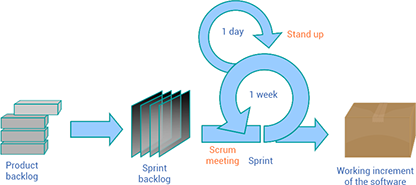
\includegraphics[width=10cm]{images/scrum-process.png}
  \caption{Illustration de la méthode Scrum\cite{scrum-process}}
\end{figure}
\ \newline
Cependant, le VideoStitch SDK et les ingénieurs y travaillant ne participent pas
aux sprints; leur travail étant plutôt organisés sous formes de missions individuelles,
en fonction des besoins des applications de l'entreprise. Ils participent toutefois 
aux \textit{stand-up} et au \textit{retrospectives}.\\
Le présent stage a suivi l'équipe dans ses sprints, en l'assistant parfois sur quelques
tickets, tout en maintenant en priorité les deux missions de fond présentées plus haut, dans 
la section présentant le sujet (section \ref{le-sujet} p.\pageref{le-sujet}).\\
\newline
Enfin, toutes les communications écrites et orales se font en anglais, du fait
de la présence dans l'équipe de personnes de langue natale espagnole, allemande ou flamande.

\section{Les outils utilisés}
